\documentclass[../master/master.tex]{subfiles}
\begin{document}
\subsection{Lockstep}
The first algorithm we will be looking at is the Lockstep algorithm (Algorithm \ref{lockstepalgo}) proposed by Bloem et al. \cite{lockstep} The Lockstep algorithm performs forward and backward search simultaneously and recurses after removal of the SCC in each iteration.

We have simplified this algorithm slightly, as we do not look at Streett automata, and are therefore not interested in the Report function introduced in the article. For the same reason, we also modified the input of the algorithm to only take a graph and a set of vertices. 

We start by initializing the set $P=V$ in the first iteration, for which we will be finding SCCs. During the iterations, this set will be modified, and once it is empty, we return, as no SCCs exist in an empty set. The algorithm then initializes the forward and backward sets \FW{v} and \BW{v} of some node $v\in P$, as well as their frontiers, which are all initially set to $\{v\}$ - the singleton set of the node picked from $P$.

The next step is simultaneously performing forward and backward set computations until either \FW{v} or \BW{v} converges. This is done by extending the forward and backward frontiers by taking their image and preimage respectively, selecting only those of the nodes, which are in our current $P$ and finally removing all the nodes which already exist in \FW{v} and \BW{v} respectively. We then update the values of \FW{v} and \BW{v} to include the elements that we have found in their respective frontiers. This is done in iterations until either of the frontiers is an empty set, meaning that it will no longer be updated.
In other words, by iteratively computing the two functions (\ref{fw}) and (\ref{bw}) until one of them reaches its least fixpoint. The forward or backward set with the empty frontier is then set as \emph{Converged}. This is essential for obtaining the $\mathcal{n \log n}$ bound we will be prove further below.

Once one of the sets has converged, we continue updating the other set, just like before until its frontier has no nodes in common with the \emph{Converged} set, as then no more nodes can be found in the SCC.
We have now found an SCC $C=\FW{v}\cap\BW{v}$. 

Now we partition the rest of $P$ into two sets: $P\setminus Converged$ and $Converged\setminus C$. To see that this is a partion of $P\setminus C$, first realize that $C\subseteq Converged$, so $P\setminus C = (P\setminus Converged) \cup (Converged\setminus C)$. It is also immediate that the two sets are disjoint, $(P\setminus Converged)\cap (Converged\setminus C)=\emptyset$. So we have a partition. Recursive calls to Lockstep on these two sets are performed; exploring each disjoint set for new SCCs. 

\begin{algorithm}[H]
  \caption{Lockstep((V, E), P $\subseteq$ V)} \label{lockstepalgo}
  \begin{algorithmic}[1]
    \Statex
    \If{$P=\emptyset$}
     \State \Return $\emptyset$
    \EndIf
    \Statex
    \Let{$v$}{pick($P$)}
    \Let{$FW, BW$, Ffront, Bfront}{$\set{v}$}
    \Statex
    \While{Ffront$\neq\emptyset$ \textbf{and} Bfront$\neq\emptyset$}
     \Let{Ffront}{$\text{img(Ffront)}\cap P\setminus FW$}
     \Let{Bfront}{$\text{preimg(Bfront)}\cap P\setminus BW$}
     \Let{$FW$}{$FW\cup\text{Ffront}$}
     \Let{$BW$}{$BW\cup\text{Bfront}$}
    \EndWhile
    \Statex
    \If{Ffront$=\emptyset$}
     \Let{$Converged$}{$FW$}
    \Else
     \Let{$Converged$}{$BW$}
    \EndIf
    \Statex
    \While{$\text{Ffront}\cap BW\neq\emptyset$ \textbf{or} $\text{Bfront}\cap FW\neq\emptyset$}
     \Let{Ffront}{$\text{img(Ffront)}\cap P\setminus FW$}
     \Let{Bfront}{$\text{preimg(Bfront)}\cap P\setminus BW$}
     \Let{$FW$}{$FW\cup\text{Ffront}$}
     \Let{$BW$}{$BW\cup\text{Bfront}$}
    \EndWhile
    \Statex
    \Let{$C$}{$FW\cap BW$}
    \Let{SCCset1}{Lockstep($(V, E)$, $Converged\setminus C$)}
    \Let{SCCset2}{Lockstep($(V, E)$, $P\setminus Converged$)}
    \Let{SCCs}{$\set{C}\cup \text{SCCset1} \cup \text{SCCset2}$}
    \State \Return SCCs
  \end{algorithmic}
\end{algorithm}

\subsection{Linear-time algorithm}
\subsubsection{Skeleton and spine-sets}
\todo[inline]{make definitions}
Gentilini et al. \cite{linear} introduce a notion of a skeleton and a spine-set, as well as a chordless path. A path is  between nodes $v_0$ and $v_p$ is chordles iff for all $0\leq i \leq j \leq p$, where $j-i>1$ and there is no edge from $v_i$ to $v_j$. In other words there can be no shortcuts - this path is the shortest in the subgraph of nodes $\{v_0, v_1, \dots, v_p\}$. 

A spine-set is a symbolic way of ordering sets of nodes. A pair \pair{S}{v} is a spine-set of $G$ iff $G$ contains a chordless path consisting of the set of vertices $S$, ending in $v$. $v$ can also be called the spine-anchor of the spine-set.

\begin{figure}[H]
\center
\begin{scaletikzpicturetowidth}{\textwidth}
\begin{tikzpicture}[scale=\tikzscale]
\begin{scope}[every node/.style={circle, fill=black, inner sep=0pt, minimum size=3mm}]
    \node (A) at (0,0) {};
    \node (B) at (3,0) {};
    \node (G) at (4.5,-1.5) {};
    \node (C) at (6,0) {};
    \node (H) at (7.5,-1.5) {};
    \node (D) at (9,0) {};
    \node[label=$v$] (E) at (12,0) {};
    \node (F) at (15,0) {};
\end{scope}

\begin{scope}[>={Stealth[black]}]
    \path [->] (A) edge  (B);
    \path [->] (B) edge (C);
    \path [->] (B) edge (G);
    \path [->] (G) edge (H);
    % \path [->] (C) edge[bend left=30]  (B);
    \path [->] (H) edge (D);
    \path [->] (C) edge  (D);
    \path [->] (D) edge  (E);
    \path [->] (E) edge  (F);
    \path [->] (E) edge[bend right=40]  (D);
    \path [->] (A) edge[bend left=30]  (F);
  \end{scope}
\draw (6,0) ellipse (7cm and 1.2cm);
\end{tikzpicture}
\end{scaletikzpicturetowidth}
\caption{Spine-set}
\label{spine}
\end{figure}

For $u, v \in V$ and a forward set \FW{v}, the pair \pair{S}{v} is a skeleton iff $u$ is also a node in $\FW{u}$ and the distance from $v$ to $u$ is maximum and $S$ is the set of nodes on the shortest path between the two vertices.
\begin{figure}[H]
\center
\begin{scaletikzpicturetowidth}{\textwidth}
\begin{tikzpicture}[scale=\tikzscale]
\begin{scope}[every node/.style={circle, fill=black, inner sep=0pt, minimum size=3mm}]
    \node[label=$u$] (A) at (0,0) {};
    \node (B) at (3,0) {};
    \node (G) at (4.5,-1.5) {};
    \node (C) at (6,0) {};
    \node (H) at (7.5,-1.5) {};
    \node (D) at (9,0) {};
    \node (E) at (12,0) {};
    \node[label=$v$] (F) at (15,0) {};
\end{scope}

\begin{scope}[>={Stealth[black]}]
    \path [->] (A) edge  (B);
    \path [->] (B) edge (C);
    \path [->] (B) edge (G);
    \path [->] (G) edge (H);
    \path [->] (H) edge (D);
    \path [->] (C) edge  (D);
    \path [->] (D) edge  (E);
    \path [->] (E) edge  (F);
    \path [->] (E) edge[bend right=40]  (D);
    \path [->] (F) edge[bend right=30]  (A);
  \end{scope}
\draw (7.5,0) ellipse (8.5cm and 1.2cm);
\end{tikzpicture}
\end{scaletikzpicturetowidth}
\caption{Skeleton}
\label{skeleton}
\end{figure}

If \FW{v} is the forward-set of $v \in V$, and if the skeleton of this forward set is \pair{S}{u}, then it is also a spine-set in $G$. We will be making use of this property in the linear-time algorithm when computing the spine-set.

\subsubsection{The algorithm}
The second algorithm we will be comparing is the linear-time algorithm \cite{linear} introduced by Gentilini et al. This algorithm takes as input a graph $G$ and spine-set $\langle S, N\rangle$, where the latter is initally set to \pair{\emptyset}{\emptyset}. Their original version of this algorithm, it outputs vertex sets of SCC subgraphs, however, we change this to return a set of SCCs, similarly to the Lockstep algorithm.

The first thing the algorithm does, is to choose for which vertex the next SCC will be computed, unless $V=\emptyset$, in which case the algorithm terminates. If $S\neq\emptyset$ and $N={v_p}$, then $v_p$ is chosen to be used in the SCC computations. Otherwise, an arbitrary node $v_i$ is chosen to act as the spine-anchor $N$.

Next, \FW{N} and a skeleton \pair{newS}{newN} on this forward-set is computed by Algorithm \ref{skelforward}. The skelForward algorithm is a helper method introduced by Gentilini et al., which computes the forward set of the given graph and the skeleton of this set. This results in the spine-set of the given graph. The next step is to determine the SCC containing $N$. We do this by checking if the set of nodes that can reach the current SCC (initially set to the singleton node in $N$) has any nodes in common with the forward set of $N$. The variable SCCs, which represents the current set of known SCCs, is then extended by the SCC that the current iteration of the algorithm has just found.

Once this is done, this procedure is called recursively on two subgraphs. The first recursive call is on the subgraph $V\setminus FW$ (its vertices and edges) as well as its spine-set, obtained by removing the SCC from the spine-set \pair{S}{N}. We then recurse again on a second subgraph, $FW\setminus SCC$ and its spine-set, \pair{newS\setminus SCC}{newN\setminus SCC}, which is found by computing the skeleton of $(V, E, N)$. Just like in the lockstep algorithm, these two sets are disjoint and do not contain the SCC found. In lines 10 and 15, we restrict the edges $E$ to correspond to the nodes $V'$ - this is written as $E \upharpoonright V'$.

\begin{algorithm}[H]
  \caption{Linear((V, E), \pair{S}{N})}
  \begin{algorithmic}[1]
    \If{$V=\emptyset$}
     \State \Return
    \EndIf
    \Statex
    \If{$S=\emptyset$}
      \Let{$N$}{pick($V$)}
    \EndIf
    \Statex
    \Let{$\langle FW, newS, newN\rangle$}{skelForward($V, E, N$)}
    \Statex
    \Let{$SCC$}{$N$}
    \While{$(\text{preimg}(SCC)\cap FW)\setminus SCC\neq\emptyset$}
     \Let{$SCC$}{$SCC\cup (\text{preimg}(SCC)\cap FW)$}
    \EndWhile
    \Statex
    \Let{$V'$}{$V\setminus FW$}
    \Let{$E'$}{$E\upharpoonright V'$}
    \Let{$S'$}{$S\setminus SCC$}
    \Let{$N'$}{$\text{preimg}(SCC\cap S)\cap(S\setminus SCC)$}
    \Let{SCCset1}{Linear($(V', E')$, \pair{S'}{N'})}
    \Statex
    \Let{$V'$}{$FW\setminus SCC$}
    \Let{$E'$}{$E\upharpoonright V'$}
    \Let{$S'$}{$newS\setminus SCC$}
    \Let{$N'$}{$newN\setminus SCC$}
    \Let{SCCset2}{Linear($(V', E')$, \pair{S'}{N'})}
    \Statex
    \Let{SCCs}{$\set{SCC}\cup \text{SCCset1} \cup \text{SCCset2}$}
    \State \Return SCCs
  \end{algorithmic}
\end{algorithm}

\begin{algorithm}[H]
  \caption{SkelForward((V, E), N)} \label{skelforward}
  \begin{algorithmic}[1]
    \Let{$L$}{$N$}
    \Statex
    \While{$L\neq \emptyset$}
    \State push(stack, $L$)
    \Let{$FW$}{$FW\cup L$}
    \Let{$L$}{img($L$)$\setminus FW$}
    \EndWhile
    \Statex
    \Let{$L$}{pop(stack)}
    \State $S' \gets N' \gets pick(L)$
    \While{stack $\neq\emptyset$}
    \Let{$L$}{pop(stack)}
    \Let{$S'$}{$S'\cup\text{pick(preimg(}S')\cap L)$}
    \EndWhile
    \Statex
    \State \Return $\langle FW, S', N' \rangle$
  \end{algorithmic}
\end{algorithm}
\subsection{Complexity}
Here, we analyze the complexity of the two algorithms. We state the results in Theorems \ref{linear} and \ref{lockstep}. For both of these proofs we charge each step to a node. We further strengthen the complexity of Linear and Lockstep in Theorem \ref{magic}.

\begin{theorem}[Following Gentilini et. al. \cite{linear}]\label{linear} Linear($V, E, \pair{\emptyset}{\emptyset}$) runs in $\mathcal{O}(|V|)$ symbolic steps.
\end{theorem}
\begin{proof} A constant number of steps is performed in lines 1-4 and 9-18, as here we call preImg once when calculating the new $N'$ for SCCset1. Each recursive call in the pseudocode (or each iterative call in our implementation) returns an SCC, and since there are at most as many SCCs as there are nodes, we can deduce that over all iterations in lines 1-4 and 9-18, the algorithm performs $\mathcal{O}(|V|)$ symbolic steps.

Next, in lines 7-8, nodes are assiged to our SCC. Since each node can be part of at most one SCC, we can also deduce that this part of the algorithm also performs $\mathcal{O}(|V|)$ symbolic steps globally.

Lastly, we have the call to skelForward in line 5, which performs the remaining symbolic steps. Here, the number of symbolic steps is the number of elements popped from the stack in skelForward before the termination of the second recursive call in the pseudocode, or before all node sets are popped from our implementation of the algorithm. Since each $v\in V$ is inserted into a spine-set at most two times within Linear($V, E, \pair{S}{N}$) \cite[p.~137-138]{linear}, we know that it will take at most $2|V|$ symbolic steps globally, and therefore we also achieve the $\mathcal{O}(|V|)$ bound for this part.

Given that each of the different parts perform $\mathcal{O}(|V|)$ symbolic steps globally, we can conclude that the algorithm runs in $\mathcal{O}(|V|)$ symbolic steps.
\end{proof}

\begin{theorem}[Following Bloem et. al. \cite{lockstep}]\label{lockstep} Lockstep($(V, E), V$) runs in $\mathcal{O}(|V|\log |V|)$ symbolic steps.
\end{theorem}
\begin{proof}
  We want to show that no more than $2 \log |V|+3$ steps per node, which gives the bound of $2|V|log|V|+3|V|$. We start by considering the number of steps and iterations for both loops, and then limit the total cost charged to a node.

  In the loop in lines 5-11 we charge 2 symbolic steps per iteration. We iterate through the loop as long as both B and F are being extended. We therefore look at the the subgraphs that result from an invocation of lockstep. We have $Converged\setminus C$, $C$ and $P\setminus Converged$. Let $S$ be the smaller of $Converged\setminus C$ and $P\setminus Converged$ and $k = |S\cup C|$.

  If $S = Converged\setminus C$, then we know that $S\cup C$ is the $Converged$ set, and since in each iteration we add at least one element to the set, we know that it takes at most $k$ iterations.

  In the other case, $S=P\setminus Converged$. Here, we know that the nodes, which are in the non-converged set at the time of termination of the loop are a subset of $S\cup C$. Therefore, the loop iterates at most $k$ times.

  In the second while loop in lines 14-18 only the non-converged set is extended. In the worst-case, this set does not contain any node from $C$ yet and must be extended by all the nodes, which will be in the SCC $C$ This gives us at most $|C|$ iterations.

  To limit the total cost per node, we consider a recursion tree R pictured in Figure \ref{R}. Each call to the algorithm corresponds to a vertex $x$ of R, where $P_x$, $S_x$ and $C_x$ are the $P$, $S$ and $C$ corresponding to that invocation. Any node $u \in V$, which we pick in line 3 of the algorithm, is only passed down one branch of the recursion tree R, as the two sets on which Lockstep is called recursively are disjoint. 3 steps are performed at the vertex in which the SCC of $u$ is found.

  We now look at the vertices in which the SCC has not been found yet. Let $x'$ be the closest descendant of $x$ where $u$ is charged again. We know that $|P_{x'}|\leq |S_x|$, as $P_{x'}$ is either $S_x$ or one of its descendants. If we take the recursion tree for $P_{x´}$, $S_{x'}$ is the smaller of the two sets and therefore $|S_{x'}|\leq |P_{x'}|/2$. Thus we also know that $|S_{x'}|\leq |S_{x}|/2$, which tells us that each node $u$ is charged at most $\log |V|$ times and an additional 3 steps when its SCC is found.

  This gives us the cost of $2|V|\ \log |V| + 3|V|$ steps, resulting in the $\mathcal{O}(|V|\log |V|)$ bound.
\end{proof}
\begin{figure}
  \centering
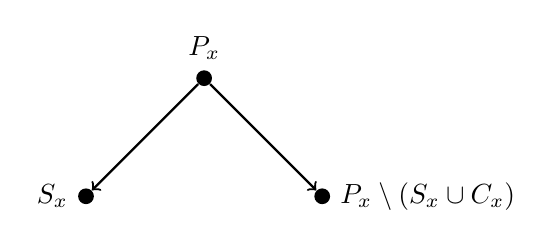
\begin{tikzpicture}[roundnode/.style={circle, fill=black, inner sep=0pt, minimum size=2mm}]
  \node[roundnode, label = $P_x$] at (0,0) (u1) {};
  \node[roundnode, label = west:$S_x$] at (-1.5 , -1.5) (u2) {};
  \node[roundnode, label = east:$P_x\setminus(S_x \cup C_x)$] at (1.5, -1.5) (u3) {};
  % Lines
  \draw[->, thick] (u1) -- (u2);
  \draw[->, thick] (u1) -- (u3);
\end{tikzpicture}
\caption{Recursion tree R}
\label{R}
\end{figure}

We can then further strengthen the bound presented above for both the linear-time and Lockstep algorithms by considering all symbolic operations.
\begin{theorem}[Following Gentilini et. al. \cite{linear}]\label{magic} Linear($V, E, \pair{\emptyset}{\emptyset}$) and Lockstep($(V, E), V$) runs in $\mathcal{O}(\text{min}(|V|, dN))$ and $\mathcal{O}(\text{min}(|V|\log|V|, dN))$ symbolic steps respectively, where $d$ is the diameter of $G$ and $N$ is the number of SCCs in $G$.\end{theorem}
\begin{proof}
  Since each call to Linear produces a new strongly connected component, the number of recursive calls is bounded by $N$. We will now show that the number of symbolic steps per iteration is bounded by $\mathcal{O}(d)$.

  By induction, we can show that for each recursive call, Linear($V_c, E_c, \pair{S_c}{N_c}$), $d_c\leq d$, where $d_c$ is the diameter of \pair{V_c}{E_c}.
  
  The base case is immediate, as we are presented with the whole graph, where $d_c=d$. We then have two cases for the inductive step:
  \begin{enumerate}
  \item $V_{c+1} = \FW[\pair{V_c}{E_c}]{v}, v\in V_c$
  \item  $V_{c+1} = V_c\setminus\FW[\pair{V_c}{E_c}]{v}, v\in V_c$
  \end{enumerate}

  In both of these cases we can show that $d_{c+1}\leq d_c$. Given two nodes $a$ to $b$, where $a, b \in V_{c+1}$ and $z$ is a node in a path of \pair{V_c}{E_c} from $a$ to $b$, then $z\in V_{c+1}$. From this, we know that for any pair of nodes $a, b\in V_{c+1}$, each path from $a$ to $b$ in \pair{V_c}{E_c} can also be found in \pair{V_{c+1}}{E_{c+1}}, and therefore $d_{c+1}\leq d_c$.
  
  For Lockstep($(V_c, E_c), P_c$), the base case is the same as for Linear and therefore $d_c=d$. The two cases for the inductive step are the following:
  \begin{enumerate}
  \item $V_{c+1} = Converged$
  \item  $V_{c+1} = V_c\setminus Converged$
  \end{enumerate}
  
  Here, $Converged$ is either $\FW[\pair{V_c}{E_c}]{v}, v\in V_c$ or $\BW[\pair{V_c}{E_c}]{v}, v\in V_c$. If $Converged = FW$, the same argument applies as for Linear, giving us $d_{c+1}\leq d_c$. If $Converged=BW$, given a path between two nodes $a, b \in V_{c+1}$ and a node $z$ on a path in \pair{V_c}{E_c} from $a$ to $b$, then \BW[\pair{V_c}{E_c}]{v} also contains this node if it contains nodes $a$ and $b$. The same argument as above follows for these two cases too, also resulting in $d_{c+1}\leq d_c$. 
  
  Since the loops in both Linear and SkelForward perform a reachability analysis, we get a bound of $\mathcal{O}(d)$ symbolic steps per recursive call. From this follows the global bound of $\mathcal{O}(dN)$. Using the bounds from Theorem \ref{linear} and \ref{lockstep}, we can further strengthen these bound respectively to $\mathcal{O}(\text{min}(|V|, dN))$ and $\mathcal{O}(\text{min}(|V|, dN))$ symbolic steps globally.
\end{proof}
\end{document}
%%% Local Variables:
%%% mode: latex
%%% TeX-master: "../master/master"
%%% End:
